\section{The laboratory notebook}
\subsection*{The aim}
\begin{frame}
  \begin{textblock*}{5cm}(2cm,0.5cm) % {block width} (coords)
  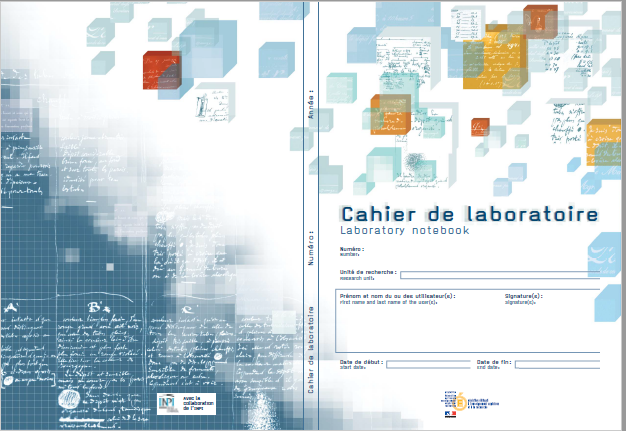
\includegraphics[width=2.3cm,height=1.3cm]{images/cahierlabo.png}
  \end{textblock*}
  \begin{textblock*}{5cm}(2cm,0.5cm) % {block width} (coords)
  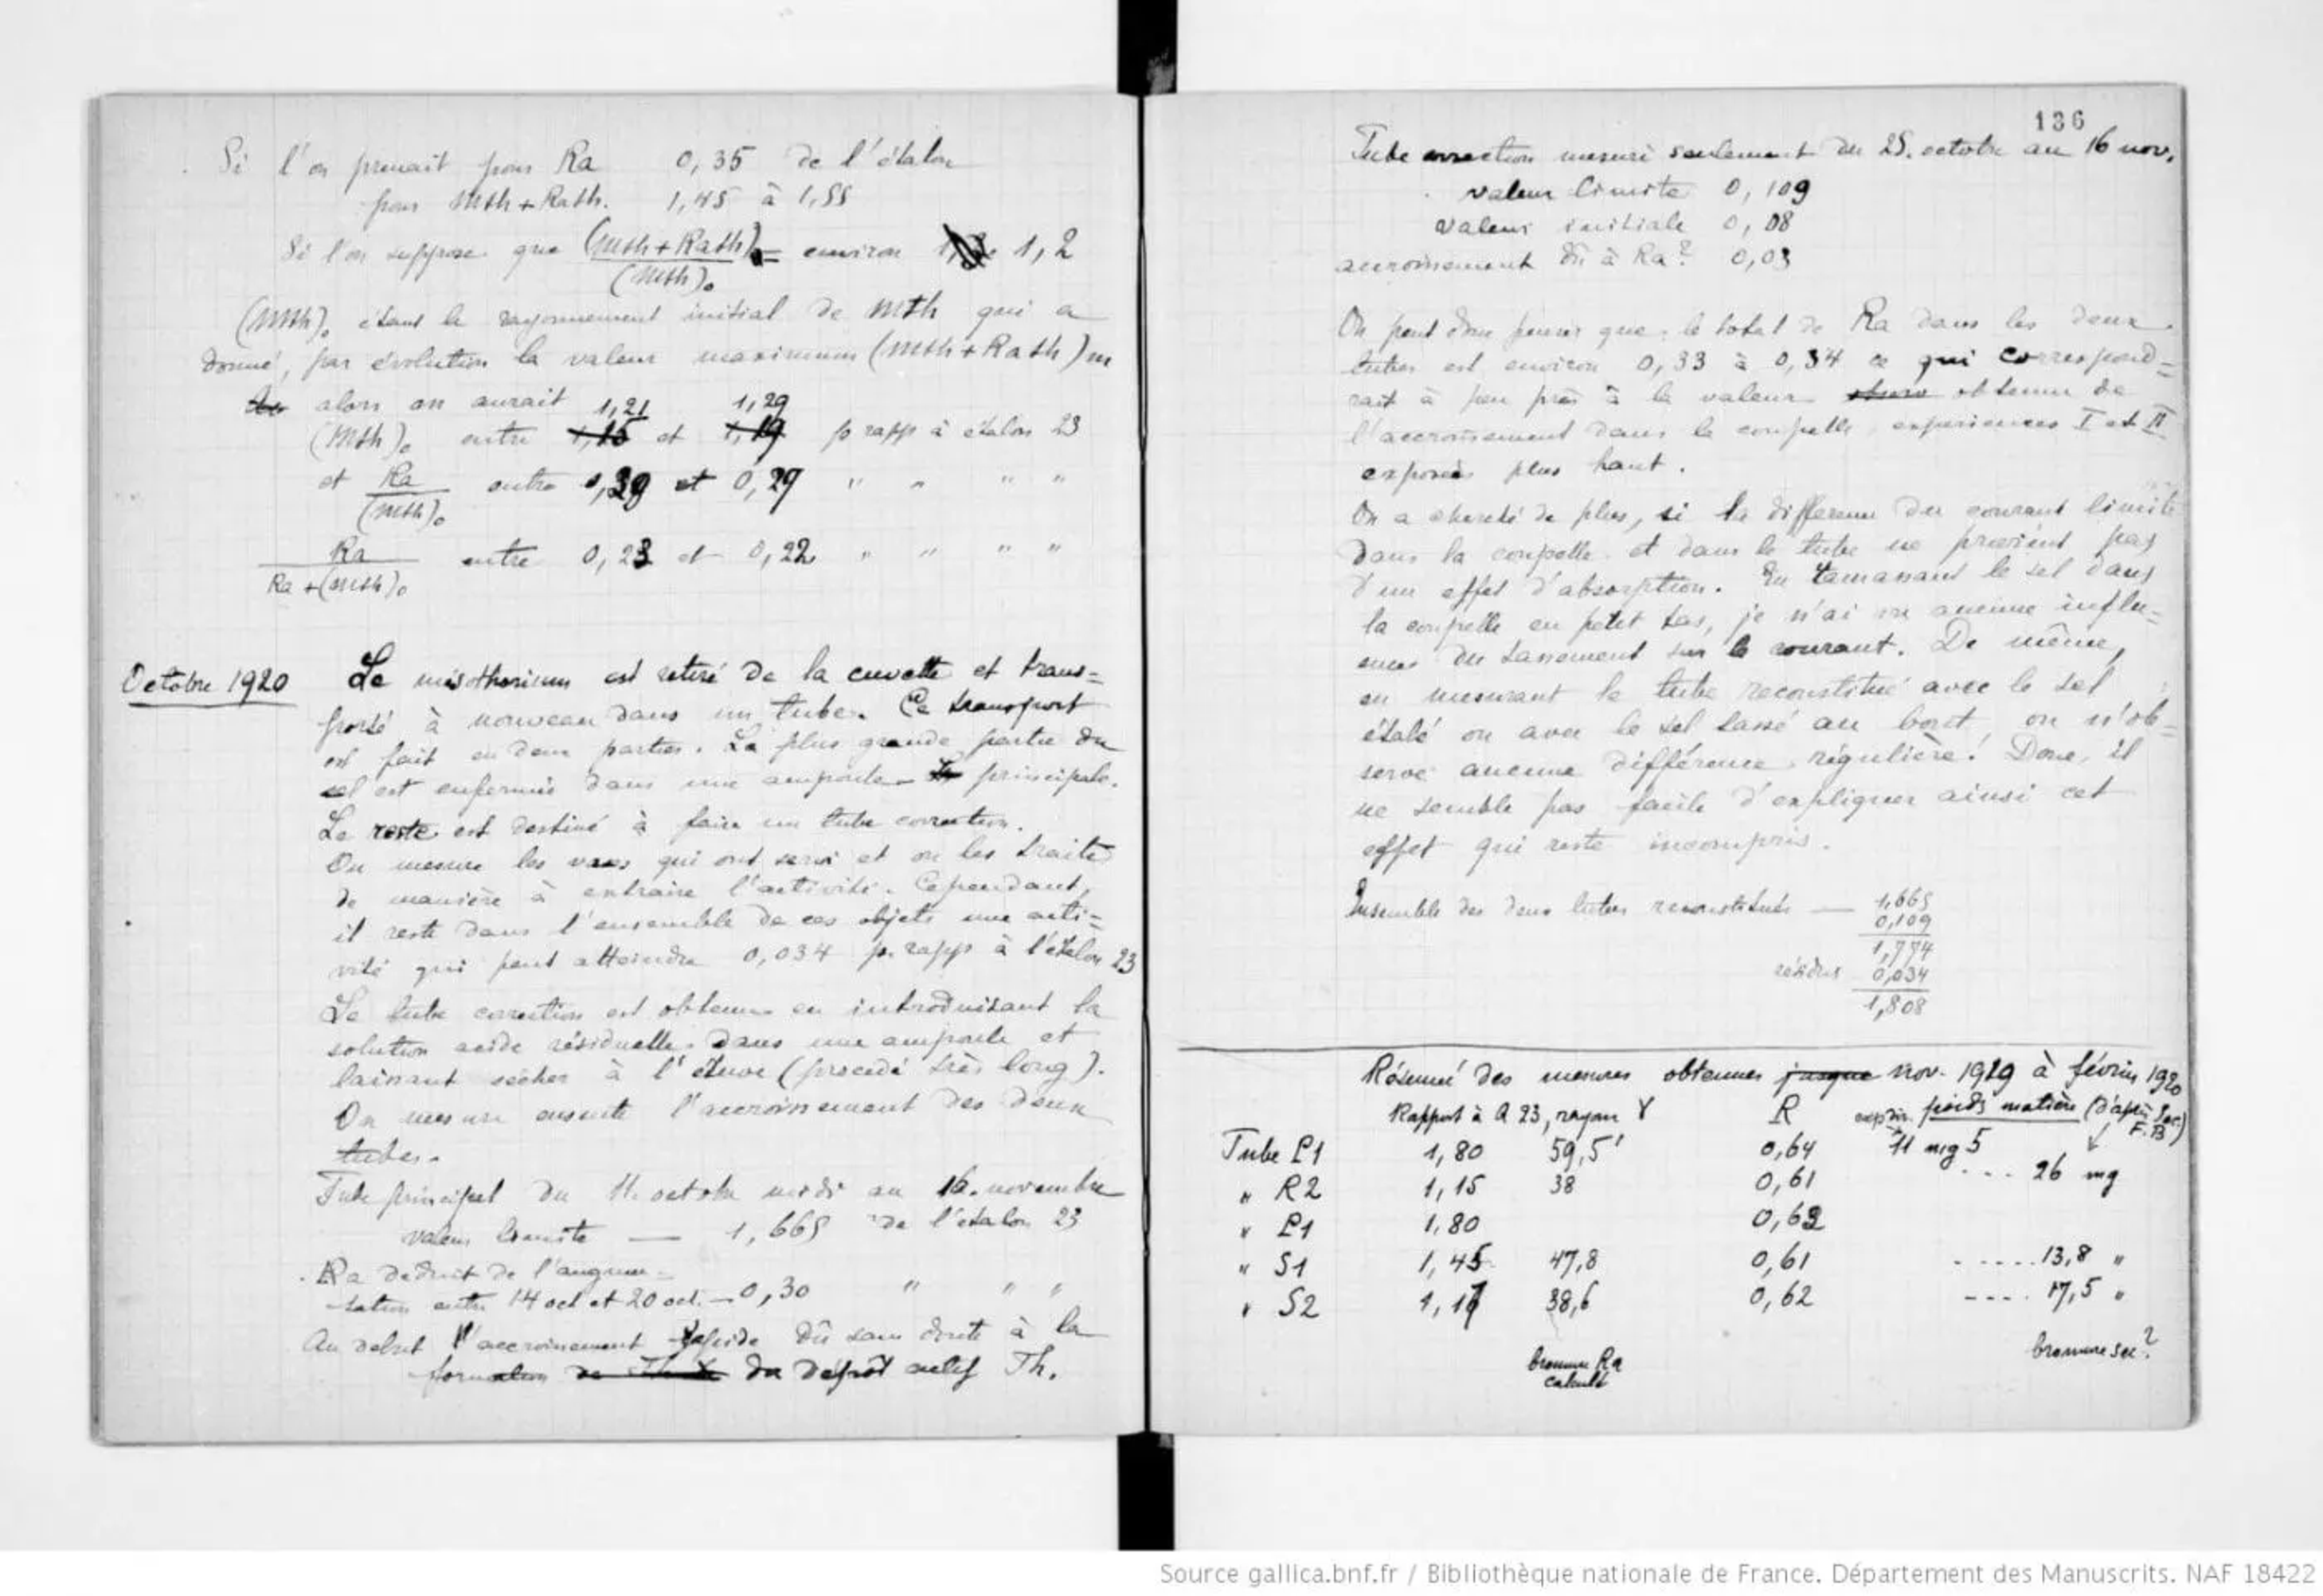
\includegraphics[width=2.3cm,height=1.3cm]{images/cahier2.pdf}
  \end{textblock*}

Laboratory notebook allow to:
\begin{itemize}
	\item Day-to-day recording each step in a process, experiments...
	\item Report on the progress, and scientific experimentations from the idea to final conclusions
	\item Keep track of knowledge in a lab
	\item Useful drafting a patent
	\item Proof of anteriority
\end{itemize}
\end{frame}

\begin{frame}{Paper version}
\begin{columns}
\column{.5\textwidth}
This is a legal tool:
 \begin{itemize}
 \item Page numbered in each notebook
 \item Cover page with the owner of the results
 \item Each page contain a part to date, to sign for at least to people
 \end{itemize}
\column{.5\textwidth}
At each research level:
  \begin{itemize}
 \item Researchers
 \item Engineers
 \item Technicians
 \item Students...
 \end{itemize}
\end{columns}
\vspace{1cm}
\centering End what's happen for bioinformatic ?
\end{frame}

\begin{frame}{Electronic version}
Electronic Laboratory Notebooks (ELN) \\
Modern LN since 2009 (C.U.R.I.E. Network) \\

\includegraphics[width=3cm,height=2cm]{images/elabftw-logo.png}
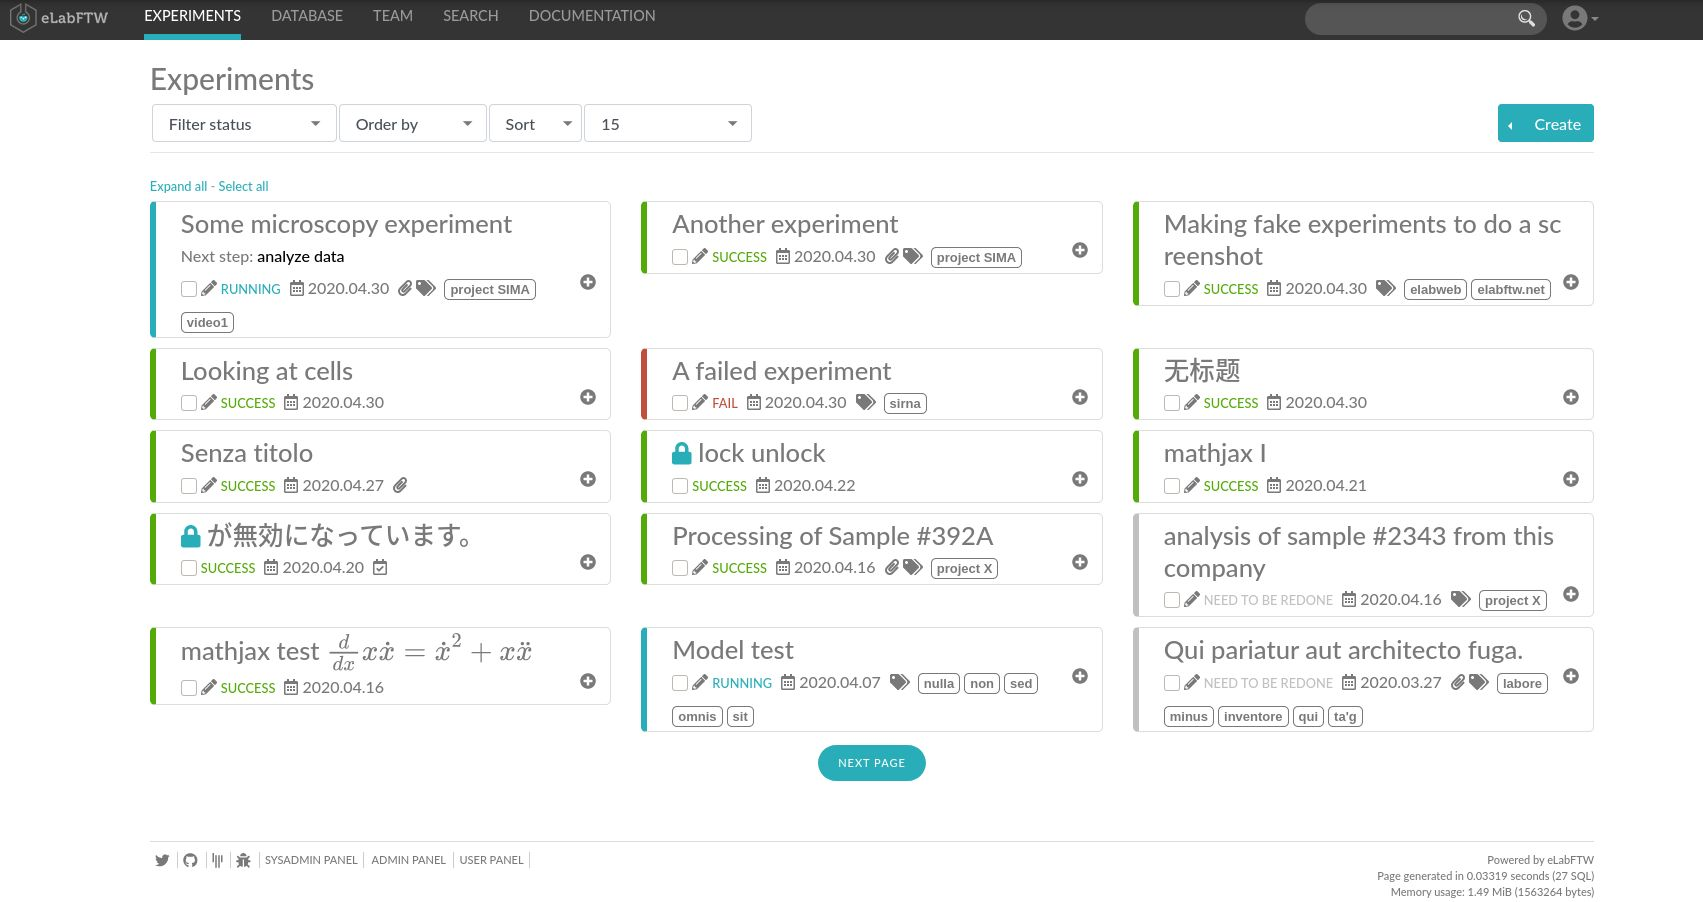
\includegraphics[width=7cm,height=3cm]{images/elabftw1.jpg}
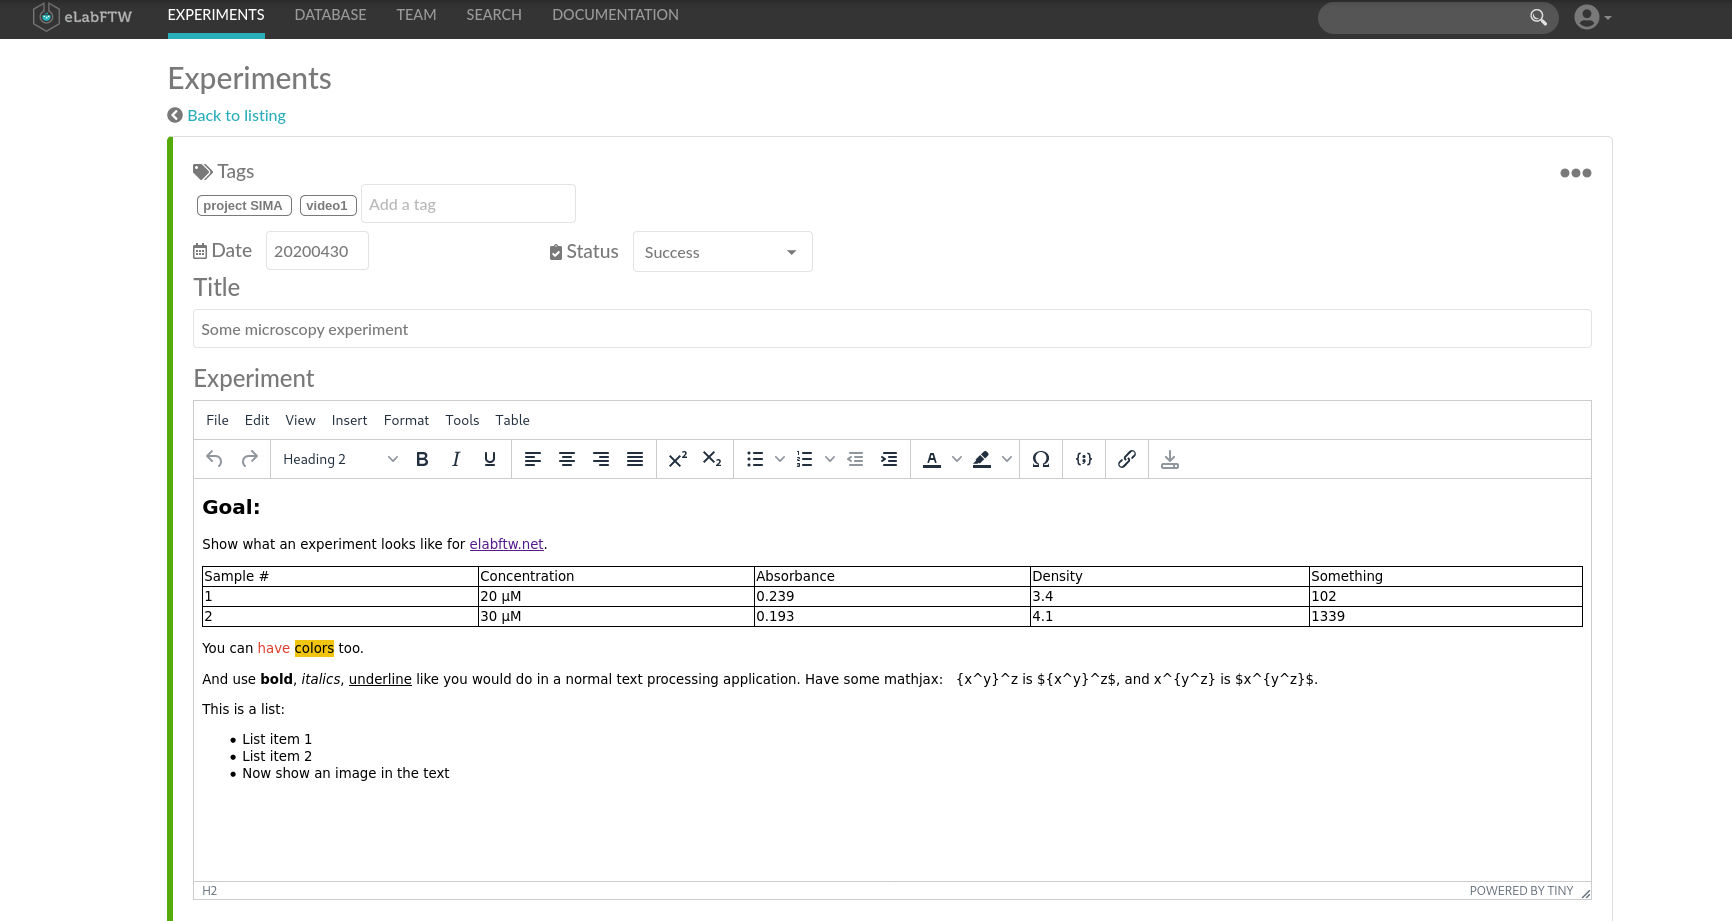
\includegraphics[width=7cm,height=3cm]{images/elabftw2.jpg}
 \begin{itemize}
 	\item dematerialised
 	\item archivable
 	\item sharable
 	\item secure
 \end{itemize}

\centering But less and less adapted to recent evolutions of our work
\centering We need an electronic tool for individual traceability
\end{frame}

\begin{frame}{Electronic version}
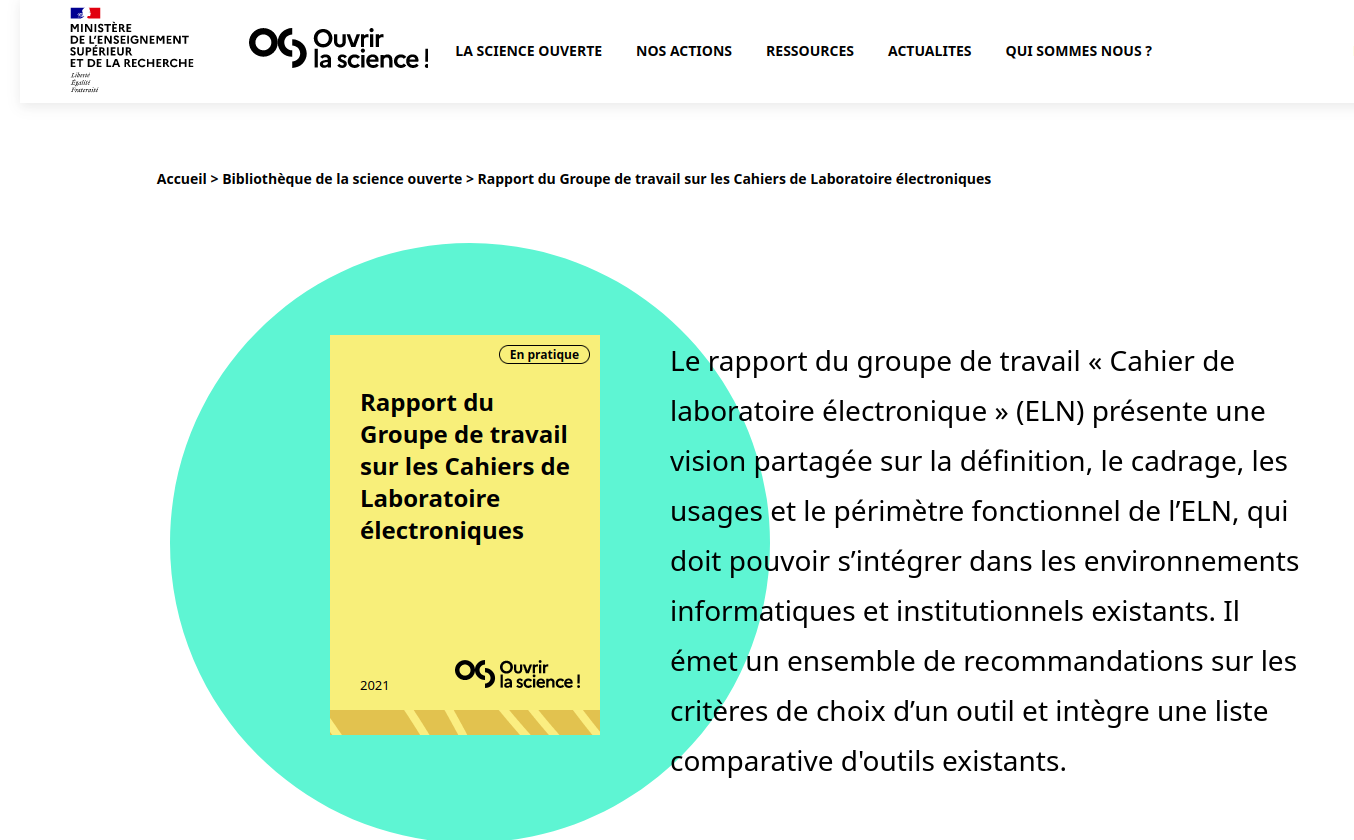
\includegraphics[width=7cm,height=3cm]{images/gt_eln.png}
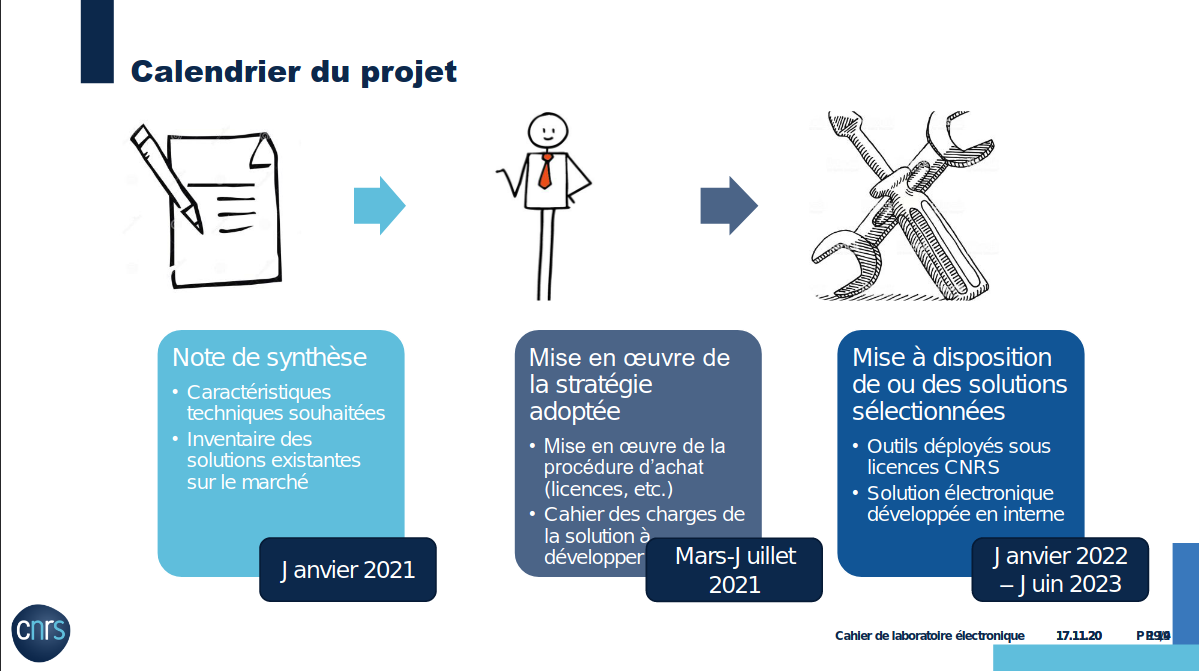
\includegraphics[width=7cm,height=3cm]{images/gt_eln_temp.png}
\end{frame}

